% Presentation on keg
%
\documentclass{beamer}
%\documentclass[handout]{beamer}
%\usepackage{beamerthemeshadow}
\usetheme{Warsaw}
\usepackage{pgf}

\pgfdeclareimage[interpolate=true,height=7cm]{faktorial}{faktorial}

\author{Michal Kov\'{a}\v{c}}
\title{User oriented language for powerful data mining with Ferda}
\date{\today}

\begin{document}
\frame{\titlepage}

\section{Introduction}
\subsection{Table of contents}
\frame{
	\frametitle{Table of contents part 1/2}
	\tableofcontents[sections={1-2},pausesections]
}

\frame{
	\frametitle{Table of contents part 2/2}
	\tableofcontents[sections={3-4},pausesections]
}

\subsection{What is Ferda Data Miner?}
\begin{frame}
	\frametitle{Ferda}
	\begin{block}{What is Ferda?}
		\begin{itemize}[<+->]
			\item User oriented application
			\item For specification of tasks, execution and result browsing
			\item Work with boxes
			\item Boxes for data mining
		\end{itemize}
	\end{block}
	\begin{block}<+->{History}
		\begin{itemize}[<+->]
			\item LISp-Miner not so much user frienly
			\item Software project at MFF 
			\item Diploma theses
		\end{itemize}
	\end{block}
\end{frame}

\begin{frame}
	\frametitle{Screenshot}
\end{frame}

\subsection{Ferda as programming language}
\begin{frame}
	\frametitle{Ferda as programming language}
\end{frame}

\subsection{What is missing? What should be done?}
\begin{frame}
	\frametitle{What is missing?}
	\begin{block}{What is missing?}
		\begin{itemize}[<+->]
			\item Moving work from one project to another
			\item Basic math boxes
			\item Recursion
			\item Other language boxes
			\item Ferda specific language boxes
			\item Data mining specific boxes for user programming
		\end{itemize}
	\end{block}	
\end{frame}


\section{New functionality in Ferda}
\subsection{Network archive}
\begin{frame}
	\frametitle{Network archive}
	\begin{block}{What is network archive?}
		\begin{itemize}[<+->]
			\item New place where user
			\item For specification of tasks, execution and result browsing
			\item Work with boxes
			\item Boxes for data mining
		\end{itemize}
	\end{block}
	
\end{frame}

\begin{frame}
	\frametitle{Screenshot -- add a connection to the network archive}
\end{frame}

\begin{frame}
	\frametitle{Screenshot -- set a name of box in the network archive}
\end{frame}

\begin{frame}
	\frametitle{Screenshot -- new box added to the network archive}
\end{frame}

\begin{frame}
	\frametitle{Screenshot -- drop box to a desktop from the n. archive}
\end{frame}

\begin{frame}
	\frametitle{Screenshot -- remove box from the network archive}
\end{frame}


\subsection{Boxes for math and the lambda function}
\begin{frame}
	\frametitle{Factorial}
	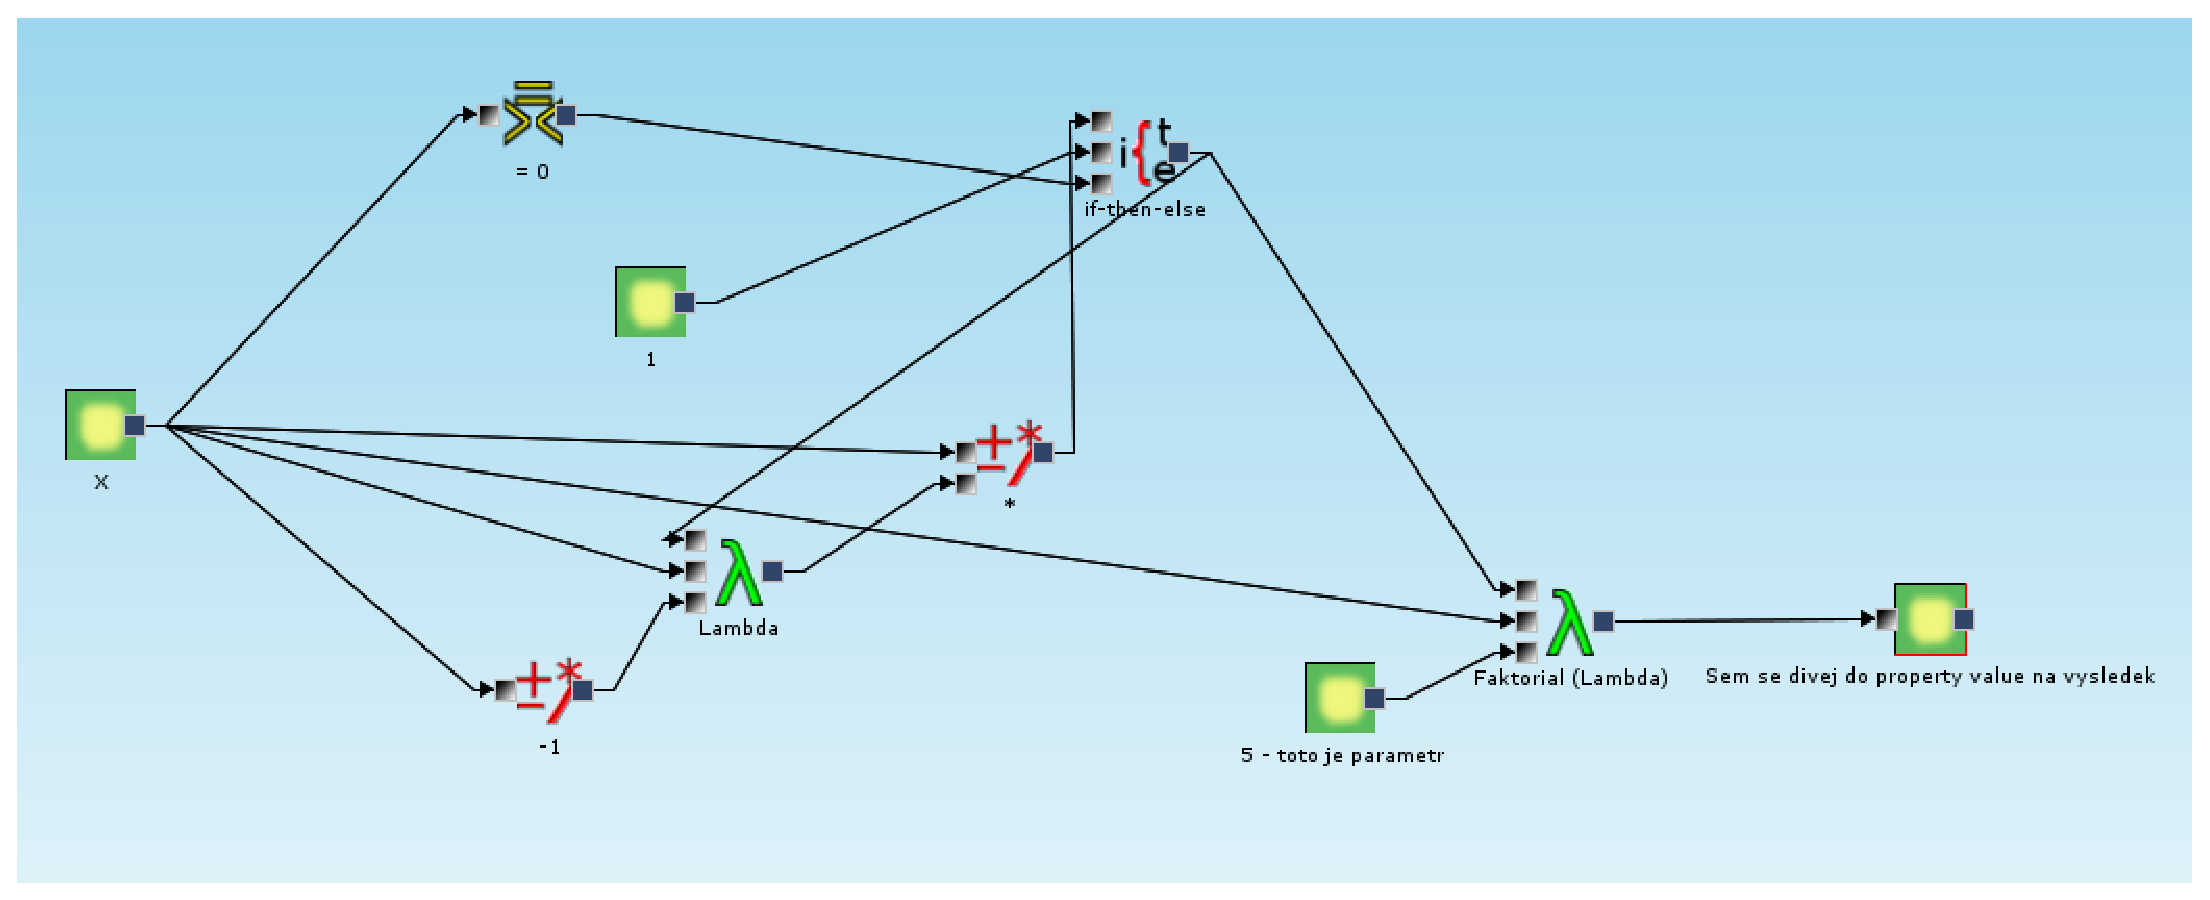
\includegraphics[interpolate=true,width=10.8cm]{faktorial}
\end{frame}
\subsection{Execute action and get parameter}
\subsection{Command and command output}

\section{Example -- executing four fold task recursively}
\subsection{Motivation}
\subsection{Linear interpolation}
\subsection{Connection of boxes}
\subsection{Results}
\begin{frame}
	\frametitle{Result}
	Text
\end{frame}

\section{Next steps}
\subsection{Sequences and sets}
\subsection{Reuse of code}
% includy, lepsi sitovy archiv, nahrani krabicek z jineho projektu
\subsection{Better lambda}
\subsection{Summary}
\frame{vitez}

\end{document}
